\chapter{Preliminares}\label{ch:Preliminares}
\section{Historia de los modelos epidemiológicos}\label{sec:Historia de la epidemiología}
De acuerdo con \cite{epiDictionary}, la epidemiología se encarga de estudiar la ocurrencia y distribución de eventos, estados y procesos relacionados con la salud de distintas poblaciones, con el objetivo de brindar estrategias de control y prevención de problemas de salud relevantes.

El primer intento por modelar teóricamente la propagación de una enfermedad, fue realizado por Daniel Bernouilli en 1760, en el cual, basándose en sus conocimientos en medicina y matemáticas, desarrolló un modelo que describe el comportamiento de la viruela y evalúa el impacto teórico de la inoculación para su época \cite{shortHistory}. 

Sin embargo, en el modelamiento epidemiológico se considera como punto de partida el modelo descrito por Kermack y McKendrick en 1927, también conocido como modelo SIR, en el que se establecen relaciones entre tres estados de una enfermedad (Susceptible-Infectado-Recuperado) y se implementan los conceptos de tasa de contagio y de recuperación \cite{malariaSIR}. Desde entonces se han desarrollado múltiples variaciones sobre el modelo SIR, con el objetivo de analizar diferentes tipos de enfermedades de una manera más precisa, considerando por ejemplo diferentes estados, tasas de natalidad y mortalidad, entre otros \cite{diego2010}.

Por otra parte y debido a los avances tecnológicos de las últimas décadas, se han desarrollado modelos y simulaciones que permiten analizar características que no eran posibles con los modelos anteriormente mencionados. Por ejemplo, patrones de movilidad \cite{colaGNN, epidemiologicalNeuralNetwork}, disminución en la cantidad de contagios debido a un aislamiento preventivo \cite{stayHome}, contagios de individuo a individuo \cite{heterogeneousPopulation} e interacciones en masa \cite{combiningGraph, transfer2021}, la mayoría realizadas con una fuerte influencia de las redes neuronales y complejas, apoyadas fuertemente sobre la teoría de grafos.

\section{Estudio epidemiológico}\label{sec:Estudio epidemiológico}
Uno de los objetos de estudio con mayor importancia en el campo de la epidemiología es la cualidad endémica de la enfermedad, es decir, si la enfermedad afectará a la población por un largo periodo de tiempo o si desaparecerá gradualmente. La manera en la que se determina está capacidad está dada por los siguientes indicadores:

\begin{itemize}
    \item \textbf{Número básico de reproducción $\mathcal{R}_0$:} Se define como la cantidad de individuos que infecta el paciente cero en una población completamente susceptible. En general, si $\mathcal{R}_0<1$ la enfermedad desaparecerá paulatinamente y sí $\mathcal{R}_0>1$, podríamos estar ante un caso de endemia.
    \item \textbf{Número de contactos adecuados $\sigma(t)$:} Es la cantidad de contactos con individuos del sistema que realiza un individuo infectado durante su etapa de infección, cuando se introduce en la población en el momento $t$.
    \item \textbf{Número de desplazamiento $\mathcal{R}(t)$:} Se entiende como la cantidad promedio de infecciones secundarias que produce un individuo infectado durante su etapa de infección, cuando es introducido en la población en el momento $t$. De ese modo, $\mathcal{R}(t) = \sigma(t)\cdot S(t)$, donde $S(t)$ indica la cantidad de individuos susceptibles en el momento $t$.
\end{itemize}

Heesterbeek y Dietz definen el número básico de reproducción $R_0$ como:
\begin{equation}\label{eq:R0}
    \mathcal{R}_0 = \int_0^\infty b(a)F(a) da,
\end{equation}
donde $b(a)$ representa la cantidad promedio de nuevos contagios que producirá un individuo infectado durante un tiempo y $F(a)$, conocida como la función de supervivencia, representa la probabilidad de que un individuo recién infectado se mantenga en ese estado durante al menos un tiempo $a$ \cite{conceptOfR0, perspectivesOnR0}.

\section{Modelos epidemiológicos clásicos}\label{sec:Modelos epidemiológicos clásicos}

Tradicionalmente, se han utilizado modelos de compartimientos para elaborar análisis epidemiológicos. En estos modelos, cada individuo perteneciente a la población de estudio es clasificado en uno de $n$ posibles ''compartimientos'', según su estado de salud.

Las siglas de cada estado del modelo definen su nombre, por ejemplo, el modelo MSEIR (\ref{fig:diagrama MSEIR}) define la interacción entre poblaciones con inmunidad "pasiva'' o temporal (M), en donde la inmunidad de los individuos se genera a partir de los anticuerpos heredados de la madre. Con la desaparición de los anticuerpos, estos individuos se vuelven susceptibles a contraer la enfermedad (S). Si un individuo susceptible entra en contacto con un individuo infectado, pasará al estado de exposición (E) en donde ya se considera infectado pero incapaz de transmitir la enfermedad. En el momento en el que el individuo adquiera la capacidad de contagiar la enfermedad, se pasará al estado (I) y finalmente, cuando el individuo se recupere y adquiera inmunidad, pasará al estado (R) del modelo.\cite{modelCompartimental}

\begin{figure}[h]
  \centering
    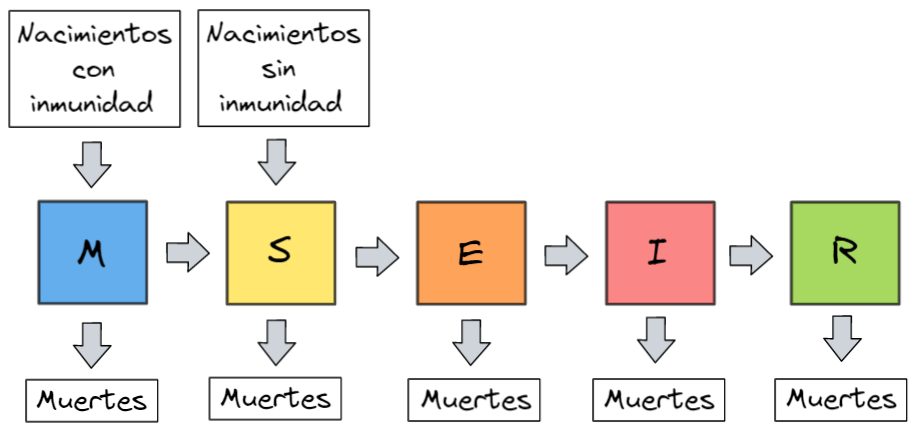
\includegraphics[width=0.7\textwidth]{Imagenes/MSEIR_compatimientos.PNG}
  \caption{Diagrama de compartimientos para el modelo MSEIR}
  \label{fig:diagrama MSEIR}
\end{figure}

Generalmente cuando hablamos de modelos epidemiológicos se consideran tres estados o clases en las que podemos dividir a la población en el tiempo: Los que pueden contraer la enfermedad, los que se infectan y los que se recuperan. Si los que se recuperan no adquieren una inmunidad permanente, nos encontraremos ante un modelo SIS, en el que los susceptibles pueden contraer la enfermedad y una vez se recuperan vuelven al estado de susceptibilidad. Por otro lado, si los individuos que se recuperan generan inmunidad a la enfermedad, estaremos ante un modelo SIR. 

Teniendo en cuenta este tipo de consideraciones nos permitimos establecer a los modelos SIS y SIR como foco principal de nuestra investigación sin dejar a un lado la idea de retomar modelos como el MSEIR para investigaciones futuras. Adicionalmente para efectos aplicables consideraremos las variaciones que tienen en cuenta la natalidad y mortalidad bien sea a causa o por efectos ajenos a la enfermedad.

Brauer y Castillo describen en \cite{mateModelsInPopulationAndEpidemiology} los planteamientos y técnicas para analizar este tipo de modelos. Nos apoyaremos también en el trabajo realizado por Diego de Pereda Sebastián en \cite{diego2010} para algunos resultados y observaciones interesantes sobre cada modelo.

\subsection{El modelo SIS}\label{sub:El modelo SIS}

El modelo SIS considera 2 posibles estados, susceptibles (S) e infectados (I). Las variaciones entre los estados vienen dadas por los nuevos contagios y los individuos que se recuperan de la enfermedad. Adicionalmente, cada estado se ve afectado por los parámetros que describen la natalidad/mortalidad y la muerte a cauda de la enfermedad. 

Los diferentes estados del modelo se pueden apreciar en el diagrama (\ref{fig:diagrama SIS}):

\begin{figure}[h]
  \centering
    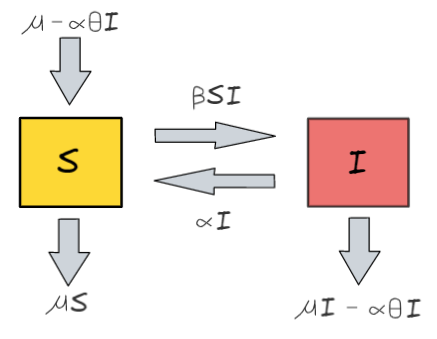
\includegraphics[width=0.4\textwidth]{Imagenes/SIS_compartimientos.PNG}
  \caption{Diagrama de compartimientos para el modelo SIS}
  \label{fig:diagrama SIS}
\end{figure}

Trabajaremos sobre una población de tamaño constante y normalizado, por lo que $S + I = 1$ y en consecuencia $S' + I' = 0$.

Normalmente cuando se habla de modelos epidemiológicos con muerte por enfermedad se consideran 4 parámetros: 

\begin{itemize}
    \item La \textbf{tasa de infección $\beta$}, que representa la probabilidad que tiene un individuo susceptible de adquirir la enfermedad luego de un contagio con un infectado.
    \item La \textbf{tasa de recuperación $\alpha$}, que podemos entender como la probabilidad de que un infectado se recupere de la enfermedad.
    \item La \textbf{tasa de natalidad/mortalidad $\mu$}, que en el caso de los modelos clásicos se supone que son iguales. La natalidad nos indica la cantidad de individuos que ingresan al espacio y la mortalidad representa los individuos que fallecen por causas ajenas a la enfermedad.
    \item La \textbf{tasa de muerte por enfermedad $\theta$}, que nos indica la probabilidad que tiene un infectado de fallecer a causa de la enfermedad.
\end{itemize}

Podemos describir el modelo a partir de un sistema de ecuaciones diferenciales como sigue:

\begin{equation}\label{eq:Modelo SIS}
\left\{
\begin{array}{l}
S' = \mu(1 - S) + (1 - \theta)\alpha I - \beta S I, \\
I' = \beta S I - (1 - \theta)\alpha I - \mu I.
\end{array}
\right.
\end{equation}

Para determinar los escenarios bajo los cuales una enfermedad es endémica debemos calcular el valor de $R_0$ para nuestro sistema de ecuaciones diferenciales (\ref{eq:Modelo SIS}). Recuerde que para determinar el valor de $R_0$ se considera una población completamente susceptible, es decir, $S=1$ e $I=0$.

Observe que los nuevos infectados vienen dados por el término $\beta S$, con lo cual definimos $b(t) = \beta S = \beta$. Por otro lado, los flujos que determinan la salida del estado de infección de los individuos viene dado por los términos $-\alpha(1-\theta)I-\mu I$, de modo que si llamamos $I(t)$ a la cantidad de individuos infectados que permanecieron infectados desde el momento $t=0$, tenemos

\begin{equation}\label{eq:Cambio en I}
\frac{dI}{dt} = -\alpha(1-\theta)I-\mu I.
\end{equation}

Si usamos el método de separación de variables obtenemos

\begin{equation}\label{eq:Infectados en el tiempo}
I(t) = I(0)e^{-(\alpha(1-\theta)+\mu)t}.
\end{equation}

De ese modo, podemos afirmar que la proporción de individuos que permanecen infectados hasta un tiempo $t$ viene dado por $e^{-(\alpha(1-\theta)+\mu)t}$, con lo cual $F(t)=e^{-(\alpha(1-\theta)+\mu)t}$. Finalmente, al reemplazar en (\ref{eq:R0}) obtenemos:

\begin{align*}
\mathcal{R}_0 &= \lim_{T\to\infty}\int_0^T b(t)F(t) dt \\
&= \lim_{T\to\infty}\int_0^T \beta e^{-(\alpha(1-\theta)+\mu)t} dt\\
&= \frac{\beta}{\alpha(1-\theta)+\mu}.
\end{align*}

\underline{\textit{Observación:}} De la ecuación (\ref{eq:Infectados en el tiempo}) podemos afirmar que la cantidad de individuos infectados tiende a cero cuando $t$ tiende a infinito.

\subsubsection{Análisis de estabilidad}

Para analizar la estabilidad de nuestro modelo SIS debemos conocer sus puntos de equilibrio. Al anular ambas derivadas nos damos cuenta de que están dados por:

$$\begin{array}{ccc}
    P_0=(S_a,I_a)=(1,0) & \text{y} & P_1=(S_b,I_b)=\left(\frac{\alpha(1-\theta)+\mu}{\beta},\frac{\beta-\alpha(1-\theta)-\mu}{\beta}\right).
\end{array}$$

Veamos que los puntos de equilibrio satisfacen las condiciones de ser positivos y menores o iguales a 1:

En el caso de $P_0$ la verificación es trivial. Por otro lado, para el caso de $P_1$ observe que 

$$0\leq\alpha(1-\theta)+\mu\leq\beta \longrightarrow \frac{\alpha(1-\theta)+\mu}{\beta}\text{, }\frac{\beta+\alpha(1-\theta)+\mu}{\beta}\geq0.$$

Si dividimos la expresión del lado izquierdo por $\beta$ obtenemos:

$$0\leq \frac{\alpha(1-\theta)+\mu}{\beta}\leq1,$$

de donde podemos afirmar que 

$$1-\frac{\alpha(1-\theta)+\mu}{\beta}\leq1 \longrightarrow \frac{\beta-\alpha(1-\theta)-\mu}{\beta}\leq1.$$

De ese modo podemos concluir que ambos puntos de equilibrio cumplen las condiciones de tener coordenadas positivas y menores que la unidad.

Es momento de determinar los comportamientos que describen ambos puntos, $P_0$ y $P_1$. Consideremos el jacobiano de nuestro modelo:

$$|A-\lambda I|=
\left|\begin{array}{cc}
-\mu-\beta I-\lambda & \lambda(1-\theta)-\beta S \\
\beta I & \beta S-\alpha(1-\theta)-\mu-\lambda
\end{array}\right|.$$

Si evaluamos en $P_0$ obtendremos los valores propios:

$$\left\{\begin{array}{l}\lambda=-\mu\text{, y}\\
\lambda=\beta-\alpha(1-\theta)-\mu.\end{array}\right.$$

Con lo que podemos afirmar que si $\mathcal{R}_0>1$, $P_0$ se comportará como un punto de silla y por otro lado, si $\mathcal{R}_0<1$ estaremos ante un nodo estable. Para el caso de $P_1$ tendremos un comportamiento tipo sumidero dado que $\lambda=0,\lambda=-\mu$ son los valores propios asociados a $P_1$.

\subsubsection{Estudio numérico}

Para representar las soluciones del sistema de ecuaciones diferenciales que describe el modelo SIS usaremos el método de Euler, el cual se implementó en el módulo: "\textit{CompartmentalModelsInEDOS}".

De manera general, dadas unas condiciones iniciales $S(0)=S_0,I(0)=I_0$ aplicamos el método de Euler a partir de la siguiente expresión:

$$\left\{\begin{array}{l}
S_{t+1} = S_t + h\cdot(\mu(1 - S_t) + (1 - \theta)\alpha I_t - \beta S_t I_t )\text{, y} \\
I_{t+1} = I_t + h\cdot(\beta S_t I_t - (1 - \theta)\alpha I_t - \mu I_t).
\end{array}\right.$$

\begin{itemize}
    \item Consideremos por ejemplo una enfermedad en la que la tasa de recuperación $\alpha$ es del $0.2$ y su tasa de infección es de $\beta=0.5$ con una tasa de letalidad de $\theta=0.4$. La tasa de natalidad para nuestra población será de $\mu=\frac{1}{75\cdot365}$, es decir, una esperanza de vida de $75$ años.
    
    \begin{figure}[h]
      \centering
        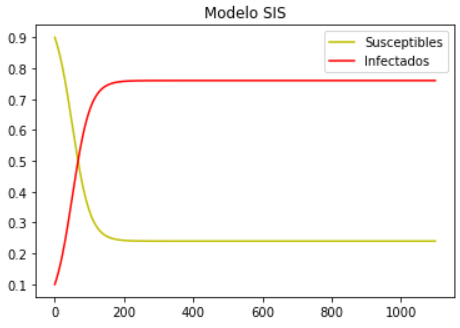
\includegraphics[width=0.4\textwidth]{Imagenes/ex1SIS.PNG}
      \caption{Evolución de la enfermedad en 1100 días con $S_0=0.9,I_0=0.1$ y $h=0.1$.}
      \label{fig:Ejemplo 1 - SIS}
    \end{figure}
\end{itemize}

\subsection{El modelo SIR}\label{sub:El modelo SIR}

Para este modelo se considera el estado de inmunidad frente a la enfermedad R. A diferencia del modelo SIS, en el modelo SIR no hay una interacción del estado I al estado S, ya que se supone que los individuos que se recuperen de la enfermedad no podrán volver a contraerla, por lo que pasaran al estado R. 

En el diagrama (\ref{fig:diagrama SIR}) se pueden apreciar las interacciones para los estados del modelo:

\begin{figure}[h]
  \centering
    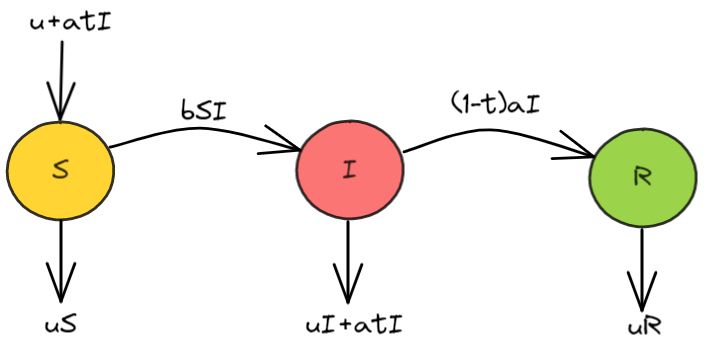
\includegraphics[width=0.7\textwidth]{Imagenes/SIR_compartimientos.PNG}
  \caption{Diagrama de compartimientos para el modelo SIR}
  \label{fig:diagrama SIR}
\end{figure}

El sistema de ecuaciones diferenciales que describe las interacciones entre estados viene dado por la siguiente ecuación:

\begin{equation}\label{eq:Modelo SIR}
\left\{
\begin{array}{l}
S' = \mu(1 - S) + \alpha\theta I - \beta S I, \\
I' = \beta S I - \mu I - \theta\alpha I - (1 - \theta)\alpha I = \beta S I - \alpha I - \mu I\text{, y } \\
R' = \alpha I - \alpha\theta I - \mu R.
\end{array}
\right.
\end{equation}

En este caso, la ecuación diferencial que describirá la cantidad de individuos infectados desde el momento 0 viene dada por:

\begin{equation}\label{eq:Infectados en el tiempo I - SIR}
    \frac{dI}{dt}=-\mu I - \alpha I \longrightarrow I(t)=I(0)e^{-(\alpha+\mu)t}.
\end{equation}

Con lo que definimos $F(t)=e^{-(\alpha+\mu)t}$. Por otra parte, la función $b(t)$ estará definida de la misma manera que en el modelo SIS debido a la manera en la que se describe el modelo. Así, al reemplazar en (\ref{eq:R0}):

\begin{align*}
\mathcal{R}_0 &= \int_0^\infty b(t)F(t) dt \\
&= \lim_{T\to\infty} \int_0^T b(t)F(t) dt \\
&= \frac{\beta}{\alpha+\mu}.
\end{align*}

\underline{\textit{Observación:}} De acuerdo con la ecuación (\ref{eq:Infectados en el tiempo I - SIR}), la población de infectada tendera a cero cuando $t$ tienda a infinito.

\subsubsection{Análisis de estabilidad}

Al igualar a cero las derivadas del sistema de ecuaciones \ref{eq:Modelo SIR} obtenemos los puntos de equilibrio:

$$\begin{array}{ccc}
P_0=(S_a,I_a,R_a)=(1,0,0) & \text{y} & P_1=(S_b,I_b,R_b)=\left(\frac{\alpha+\mu}{\beta},\frac{\mu(\beta-\alpha-\mu)}{\beta(\mu+(1-\theta)\alpha)},\frac{(1-\theta)\alpha(\beta-\alpha-\mu)}{\beta(\mu+(1-\theta)\alpha)}\right).
\end{array}$$

Veamos que las coordenadas de ambos puntos cumplen las condiciones de ser positivos y menores o iguales que uno: 

En el caso de $P_0$ se cumple de manera trivial. Por otro lado, como $\alpha,\beta,\theta$ y $\mu$ son valores positivos podemos afirmar que $S_b>0$, para $I_b$ y $R_b$ observe que 

$$\begin{array}{ccc}
\frac{\mu(\beta-\alpha-\mu)}{\beta(\mu+(1-\theta)\alpha)},\frac{(1-\theta)\alpha(\beta-\alpha-\mu)}{\beta(\mu+(1-\theta)\alpha)}>0 & \text{, si} & \beta-\alpha-\mu>0.
\end{array}$$

De la ecuación anterior podemos afirmar que 

$$\beta-\alpha-\mu>0\longrightarrow1>\frac{\alpha+\mu}{\beta}.$$

Además, como ya sabemos que se trata de un valor positivo podemos deducir que 

\begin{align*}
1&>1-\frac{\alpha+\mu}{\beta} \\
&= \frac{(\beta-\alpha-\mu)(\mu+(1-\theta)\alpha)}{\beta(\mu+(1-\theta)\alpha)}\\
&= \frac{\mu(\beta-\alpha-\mu)}{\beta(\mu+(1-\theta)\alpha)}+\frac{(1-\theta)\alpha(\beta-\alpha-\mu)}{\beta(\mu+(1-\theta)\alpha)}.
\end{align*}

Así,

$$\frac{\mu(\beta-\alpha-\mu)}{\beta(\mu+(1-\theta)\alpha)},\frac{(1-\theta)\alpha(\beta-\alpha-\mu)}{\beta(\mu+(1-\theta)\alpha)}<1.$$

Hemos demostrado que ambos puntos de equilibrio cumplen con las condiciones de tener coordenadas positivas y menores a la unidad. Ahora analizaremos la estabilidad de nuestro modelo SIR, consideremos el jacobiano de nuestro sistema de ecuaciones diferenciales:

$$|A-\lambda I|=(-\mu-\lambda)
\left|\begin{array}{cc}
-\beta I-\mu-\lambda & -\beta S+\theta\alpha\\
\beta I & \beta S-\alpha-\mu -\lambda
\end{array}\right|.$$

Si evaluamos en el punto $P_1$, podemos identificar un comportamiento de tipo silla si $\beta-\alpha-\mu>0$, en caso contrario nos encontraremos ante un nodo estable. Si tomamos ahora el punto $P_2$ y observamos los valores propios:

$$\left\{\begin{array}{l}
\lambda=-\mu,\\
\lambda=-\frac{1}{2}\frac{\mu\beta-\mu\theta\alpha+\sqrt{(\mu\beta-\mu\theta\alpha)^2-4\mu(\beta-\alpha-\mu)(\alpha+\mu-\theta\alpha)^2}}{\alpha+\mu-\theta\alpha} \text{, y}\\
\lambda=-\frac{1}{2}\frac{\mu\beta-\mu\theta\alpha-\sqrt{(\mu\beta-\mu\theta\alpha)^2-4\mu(\beta-\alpha-\mu)(\alpha+\mu-\theta\alpha)^2}}{\alpha+\mu-\theta\alpha}.
\end{array}\right.$$

De ese modo obtendremos dos tipos de comportamientos: una espiral estable si los valores propios son imaginarios y un nodo estable en el caso de que los valores propios sean reales.

\subsubsection{Estudio numérico}

De manera general, si usamos el método de Euler dadas las condiciones iniciales $S(0)=S_0,I(0)=I_0$ y $R(0)=R_0$ las expresiones que describen las soluciones discretas son:

$$\left\{\begin{array}{l}
S_{t+1} = S_t + h\cdot(\mu(1 - S_t) + \alpha\theta I_t - \beta S_t I_t), \\
I_{t+1} = I_t + h\cdot(\beta S_t I_t - \alpha I_t - \mu I_t)\text{, y} \\
R_{t+1} = R_t + h\cdot(\alpha I_t - \alpha\theta I_t - \mu R_t).
\end{array}\right.$$

\begin{itemize}
    \item Para este ejemplo supondremos una variación de la enfermedad contemplada en el ejemplo del modelo SIS en la que los individuos que se recuperan de la enfermedad adquieren inmunidad.
    
    \begin{figure}[h]
      \centering
        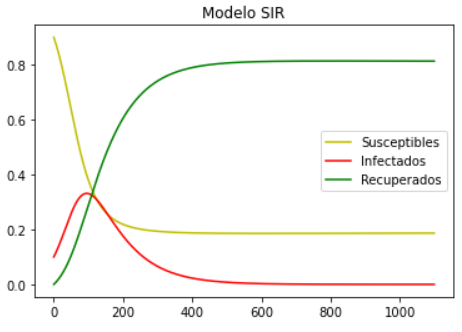
\includegraphics[width=0.4\textwidth]{Imagenes/ex1SIR.PNG}
      \caption{\centering Evolución de la enfermedad en 1100 días con $S_0=0.9,I_0=0.1,R_0=0$ y $h=0.1$.}
      \label{fig:Ejemplo 1 - SIR}
    \end{figure}
\end{itemize}

\section{Algunos conceptos de topología}\label{sec:Algunos conceptos de topología}

Empezaremos esta sección con algunas definiciones y propiedades básicas de topología, pasando por conceptos como el de base y de vecindad para luego exponer dos proposiciones para la construcción de topologías a partir de sub colecciones de la familia de partes de un conjunto y finalmente hablaremos de propiedades de orden y numerabilidad para el enfoque de nuestro proyecto. Para esto nos apoyaremos en los conceptos expuestos por Munkres en \cite{munkres}, Casarrubias y Tamariz en \cite{elementosTopologiaGeneral}, Macho en \cite{stadler2002}, Neira en \cite{NeiraNacional} y Barmak en \cite{barmak2011}.

\textbf{Definición 1.4.1:} Una \textit{topología} sobre un conjunto $X$ es una colección $\tau$ de subconjuntos de $X$ que satisface las siguientes condiciones:
\begin{enumerate}
    \item $\emptyset$ y $X$ están en $\tau$,
    \item si $A,B\in\tau$, entonces $A\cap B\in\tau$, y 
    \item la unión de cualquier subcolección de $\tau$ esta en $\tau$.
\end{enumerate}
Los elementos de $\tau$ se conocen como \textit{abiertos} de $X$ y la pareja $(X,\tau)$ es llamada como un \textit{espacio topológico}. Es común encontrar menciones a $X$ como un espacio topológico, esto se hace solo si el contexto es lo suficientemente claro como para omitir a $\tau$ de la escritura.

\begin{itemize}
    \item \textbf{Ejemplo 1.4.2:} Sea $X$ un conjunto cualquiera. La familia de todos los subconjuntos de $X$ es una topología sobre $X$ y es llamada la \textit{topología discreta} de $X$.
\end{itemize}

En ocasiones describir específicamente la topología de un conjunto es una tarea bastante compleja. Para evitar este tipo de inconvenientes se especifica una colección más pequeña de subconjuntos de $X$ llamada base de la topología sobre $X$, que es capaz de definir dicha topología. 

\textbf{Definición 1.4.3:} Una \textit{base} para una topología sobre un conjunto $X$ es una colección $\mathcal{B}$ de subconjuntos de $X$ tales que:
\begin{enumerate}
    \item Para todo $x\in X$, existe $B\in\mathcal{B}$ tal que $x\in B$, y
    \item dados $B_1,B_2\in\mathcal{B}$, existe $B_3\in\mathcal{B}$ tal que $B_3\subseteq B_1\cap B_2$.
\end{enumerate}
Los elementos de $\mathcal{B}$ son llamados elementos básicos de $\mathcal{B}$.

\begin{itemize}
    \item \textbf{Ejemplo 1.4.4:} La colección de conjuntos unipuntuales de cualquier conjunto $X$ forma una base para la topología discreta de $X$.
\end{itemize}

\textbf{Definición 1.4.5:} Sean $X$ un espacio topológico y $x\in X$. Diremos que un subconjunto $V$ de $X$ es una \textit{vecindad} de $x$ si existe un abierto $A$ tal que $x\in A\subseteq V$. Denotaremos por $\mathcal{V}(x)$ a la familia de todas las vecindades de $x$.

Esta definición nos permite realizar la siguiente afirmación:

\textbf{Teorema 1.4.6:} Un subconjunto $A$ de un espacio topológico $X$ es un conjunto abierto si, y solo si es vecindad de cada uno de los puntos que contiene.

\begin{proof}
La primera implicación se obtiene del hecho de que $A$ es abierto y $A\subseteq A$. Por otra parte, si suponemos que $A$ es vecindad de cada uno de sus puntos podemos afirmar que para cada $x\in A$ existe un abierto $V_x$ tal que $x\in V_x\subseteq A$. Veamos que $A=\bigcup_{x\in A}V_x$:

$(\supseteq)$ Se obtiene de manera trivial por la definición de los conjuntos $V_x$.

$(\subseteq)$ Sea $x\in A$. Ya que $A$ es vecindad de cada uno de sus puntos existe $V_x$ tal que $x\in V_x\subseteq A$, de modo que $x\in V_x\subseteq\bigcup_{x\in A}V_x$. Con lo que concluimos la igualdad.
\end{proof}

La siguiente proposición resume las propiedades más importantes de las vecindades:

\textbf{Proposición 1.4.7:} Sea $X$ un espacio topológico, entonces para cada $x\in X$:
\begin{enumerate}
    \item Si $U\in\mathcal{V}(x)$, entonces $x\in U$,
    \item si $U,V\in\mathcal{V}(x)$, entonces $U\cap V\in\mathcal{V}(x)$,
    \item para cada $U\in\mathcal{V}(x)$, existe $V\in\mathcal{V}(y)$ tal que $U\in\mathcal{V}(y)$ para cada $y\in V$, y 
    \item si $U\in\mathcal{V}(x)$ y $U\subseteq V\subseteq X$ entonces $V\in\mathcal{V}(x)$.
\end{enumerate}

\begin{proof} $$$$
\begin{enumerate}
    \item Se verifica directamente de la definición de vecindad. 
    \item Sean $A,B\in\tau$ tales que $x\in A\subset U$ y $x\in B\subset V$, luego $x\in A\cap B\subseteq U\cap V$, con $A\cap B\in\tau$. De ese modo, por la definición de vecindad se concluye que $U\cap V\in\mathcal{V}(x)$.
    \item Sea $U\in\mathcal{V}(x)$. Entonces existe $V\in\tau$ tal que $x\in V\subseteq U$.
    
    Dado que $V$ es abierto, por el teorema 1.4.6 se cumple que $V\in\mathcal{V}(x)$. Además, si $y\in V$ entonces $y\in V\subseteq U$ y $V\in\tau$ por lo que $U\in\mathcal{V}(y)$ para $y\in V$ arbitrario.
    \item Sea $U\in\mathcal{V}(x)$, luego existe $A\in\tau$ tal que $x\in A\subseteq V$, además como $A\in\mathcal{\tau}$ aplicamos la definición de vecindad y tenemos $V\in\mathcal{V}(x)$.
\end{enumerate} 
\end{proof}

Así como una base de una topología $\tau$ contiene toda la información necesaria para generarla, también podemos tomar de manera conveniente alguna subcolección de $\mathcal{V}(x)$ que guarde la información topológica necesaria para generar a $\mathcal{V}(x)$.

\textbf{Definición 1.4.8:} Para un punto $x$ en un espacio topológico $X$ un subconjunto $\mathcal{B}(x)$ de $\mathcal{V}(x)$ es un \textit{sistema fundamental de vecindades de $x$} sí para cada $V\in\mathcal{V}(x)$, existe $B\in\mathcal{B}(x)$ tal que $B\subseteq V$. Los elementos de $\mathcal{B}(x)$ son llamados \textit{vecindades (o entornos) básicos} de $x$.

Esta definición nos motiva a pensar en los métodos para contruir topologías sobre un conjunto $X$ con propiedades particulares. A continuación mostraremos dos de ellos:

\textbf{Proposición 1.4.9:} Sea $\mathcal{B}$ una familia de subconjuntos de un conjunto $X$ que satisface:
\begin{enumerate}
    \item $X=\bigcup \mathcal{B}$, y 
    \item si $B_1,B_2\in\mathcal{B}$ y $x\in B_1\cap B_2$, entonces existe $B\in\mathcal{B}$ tal que $x\in B\subseteq B_1\cap B_2$.
\end{enumerate}
Entonces la colección $\tau_\mathcal{B}=\{A\subseteq X:\exists\mathcal{A}\subseteq\mathcal{B}\text{ con }A=\bigcup\mathcal{A}\}$ es una topología sobre $X$ que contiene a $\mathcal{B}$ como base.
\begin{proof}
Claramente $\emptyset$ y $X$ estan en $\tau_\mathcal{B}$. Considere ahora los conjuntos $A_1,A_2\in\tau_\mathcal{B}$ y veamos que su interesección es un elemento en $\tau_\mathcal{B}$: Si $A_1\cap A_2=\emptyset$ la propiedad se deduce del caso anterior. Supongamos que $A_1\cap A_2\neq\emptyset$, luego para $x\in A_1\cap A_2$ existen $B_1,B_2\in\mathcal{B}$ tales que $x\in B_1\cap B_2$ y $B_1\subseteq A_1, B_2\subseteq A_2$ con $A_i=\bigcup B_i$ para $B_i\in\mathcal{B}$ e $i\in\{1,2\}$. Así, de (2) podemos afirmar que existe $B_x\in\mathcal{B}$ tal que $B_x\subseteq B_1\cap B_2$. De manera análoga a la demostración de la igualdad de conjuntos del teoréma 1.4.6 podemos afirmar que: 
$$A_1\cap A_2=\bigcup\{B_x:x\in A_1\cap A_2\}.$$
Para demostrar el inciso 3 en la definición 1.4.1 considere una subcolección $\mathcal{A}\subset\tau_\mathcal{B}$ y observe que
\begin{align*}
    \bigcup\mathcal{A} &= \bigcup\{A:A=\bigcup\mathcal{C}\text{ con }A\in\mathcal{A}\text{ y }\mathcal{C}\subseteq\mathcal{B}\}\\
    &= \bigcup\{\bigcup\mathcal{C}:\bigcup\mathcal{C}\in\mathcal{A}\text{ y }\mathcal{C}\subseteq\mathcal{B}\}\\
    &= \bigcup\{\mathcal{C}:\bigcup\mathcal{C}\in\mathcal{A}\text{ y }\mathcal{C}\subseteq\mathcal{B}\}.
\end{align*}
Por lo tanto $\bigcup\mathcal{A}\in\tau_\mathcal{B}$.
\end{proof}

\textbf{Proposición 1.4.10:} Si para cada $x\in X$ se elige una familia $\mathcal{V}(x)\neq\emptyset$  de subconjuntos de $X$ de tal forma que las colecciones $\mathcal{V}(x)$ cumplen:
\begin{enumerate}
    \item Si $U\in\mathcal{V}(x)$, entonces $x\in U$,
    \item si $U,V\in\mathcal{V}(x)$, entonces $U\cap V\in\mathcal{V}(x)$,
    \item para cada $U\in\mathcal{V}(x)$, existe $V\in\mathcal{V}(x)$ tal que $U\in\mathcal{V}(y)$ para cada $y\in V$, y 
    \item Si $U\in\mathcal{V}(x)$ y $U\subseteq V\subseteq X$, entonces $V\in\mathcal{V}(x)$,
\end{enumerate}
entonces la familia $\tau=\{\emptyset\}\cup\{A\subseteq X:\text{para cada }x\in A\text{ existe }V\in\mathcal{V}(x)\text{ con }V\subseteq A\}$ es un sistema de vecindades de $x$ para esta topología.

\begin{proof}
Demostraremos primero que $\tau$ es una topología: Por la definición de $\tau$ tenemos $\emptyset\in\tau$. Si tomamos $x\in X$ sabemos que existe $U\in\mathcal{V}(x)$, en particular $U\subseteq X$ y de ese modo $X\in\tau$. Considere ahora $A_1,A_2\in\tau$ y $x\in A_1\cap A_2$, luego por hipotésis existen $U_1,U_2\in\mathcal{V}(x)$ tales que $x\in U_1\subseteq A_1$ y $x\in U_2\subseteq A_2$. Del inciso (2) se tiene que $U_1\cap U_2\in\mathcal{V}(x)$ y como $x\in A_1\cap A_2$ se afirma que $U_1\cap U_2\subseteq A_1\cap A_2\in\tau$. Para mostrar el (3) inciso de la definición de topología, considere $\mathcal{A}\subseteq\tau$ y $x\in\bigcup\mathcal{A}$, entonces existe $A\in\mathcal{A}$ tal que $x\in A$. Como $A\in\tau$ existe $U\in\mathcal{V}(x)$ tal que $x\in U\subseteq A$. De lo anterior y del hecho de que $U\subseteq\bigcup\mathcal{A}$, concluimos que $\bigcup\mathcal{A}\in\tau$ y por lo tanto $\tau$ es una topología sobre $X$.

Para demostrar que $\mathcal{V}(x)$ es el sistema fundamental de vecindades veamos primero que es una familia de vecindades: Tome $U\in\mathcal{V}(x)$ y $A=\{y\in U:U\in\mathcal{V}(y)\}\in\tau$. Luego, para $a\in A$ se cumple que $a\in U$ y $U\in\mathcal{V}(a)$. De la condición (3) se sabe que existe $V_a\in\mathcal{V}(a)$ tal que $U\in\mathcal{V}(y)$ para cada $y\in V_a$. De la definición de $A$ se cumple que $V_a\subseteq A$ y de la cuarta condición podemos afirmar que $A\in\mathcal{V}(a)$, con lo cual $A\in\tau$. Se concluye que $U$ es vecindad de $x$ y $\mathcal{V}(x)$ es una familia de vecindades de $x$.

Finalmente, para una vecindad $U$ de $x$ existe $V\in\tau$ tal que $x\in V\subseteq U$ por la definición de vecindad. Luego $V\in\mathcal{V}(x)$ y así, $\mathcal{V}(x)$ es sistema fundamental de vecindades en $(X,\tau)$.
\end{proof}

Es natural pensar en que si consideramos un sistema de vecindades $\mathcal{V}(x)$ se establezca una relación de orden parcial con los demás elementos. Teniendo esto en mente definimos los siguientes conceptos:

\textbf{Definición 1.4.11:} Una \textit{vecindad minimal de} $x$ es la intersección de todas las vecindades de $x$. Lo denotaremos como $U_x$.

\textbf{Proposición 1.4.12:} La unión de todas las vecindades minimales $U_x$ para $x\in X$ forma una base para la topología de $X$. Esta base es llamada \textit{base minimal}.

Es facil ver que cualquier otra base de la topología sobre $X$ continene a la base minimal y esto a su vez garantiza que es una base para lo topología.

\textbf{Definición 1.4.13:} Un \textit{conjunto preordenado finito} es un conjunto finito con una relación transitiva y reflexiva. Definiremos el la relación de orden parcial $x\preceq y$ si $x\in U_y$.

\textbf{Definición 1.4.14:} Un elemento $x$ en un conjunto parcialmente ordenado es llamado un maximal si $y\succeq x$ implica $y=x$, y es un máximo si $y\preceq x$ para todo $y\in X$.

\textbf{Definición 1.4.15:} Un espacio topológico $X$ es $T_0$ si para cada par de puntos $x,y\in X$ con $x\neq y$, existe $V\in\mathcal{V}(x)$ tal que $y\notin V$.

\textbf{Definición 1.4.16:} Un espacio topológico $X$ que tiene un sistema fundamental de vecindades numerable en cada uno de sus puntos se dice que satisface el primer axioma de numerabilidad o simplemente que es uno-numerable.

\section{Autómatas celulares}\label{sec:Autómatas celulares}

Los autómatas celulares nacen con el trabajo de Von Neumann a finales de la década de 1940 con su trabajo \textit{"The General and Logical Theory of Automata"} en el que se plantean por primera vez las ideas para una máquina capaz de autorreplicarse. Trabajó sobre un sistema bidimensional discreto para desarrollar dinámicas bastante complejas que además fueran autorreplicables \cite{alfons2010,ACaplicacionesComputacion}.

De acuerdo con \cite{descripcionyAplicaciones}, podemos pensar en un autómata celular como un conjunto de células que tienen diferentes comportamientos en el tiempo y que interactúan entre sí, de la misma manera que en sistema biológico de donde se obtiene su nombre.

La implementación computacional de un autómata celular por lo general se hace sobre matrices, por lo que el sistema que se quiere modelar se describe sobre una malla de tamaño regular, como en la figura (\ref{fig:AC a matriz}). Una vez se definen las características de cada célula y sus relaciones con las demás se establece una equivalencia con un conjunto de valores o caracteres que conoceremos como estados del autómata y finalmente, sobre esos estados definiremos las reglas de comportamiento para nuestro modelo.

\begin{figure}[h]
  \centering
    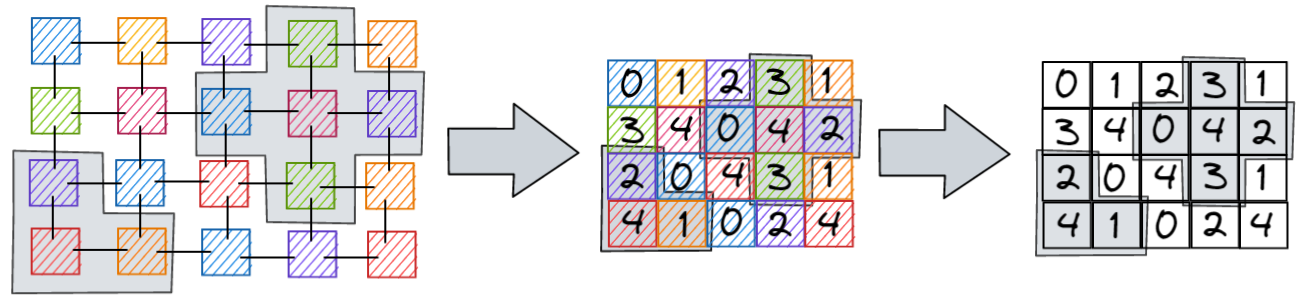
\includegraphics[width=1\textwidth]{Imagenes/ACaMatriz.PNG}
  \caption{Implementación computacional clásica de un autómata celular}
  \label{fig:AC a matriz}
\end{figure}

A continuación definiremos los elementos que componen a un autómata celular:

\subsubsection{Espacio de células}

Un espacio de células $\mathcal{L}$ es el conjunto donde viven e interactuan todas las células que se consideran para el modelo. En general este espacio es discreto, regular y finito, esto último debido a las limitaciones computacionales con las que se construyen los modelos en autómatas celulares.

La conición de regularidad de nuestro espacio de células se refiere a que las celdas que lo conforman se organizan de una manera regular, con lo que podemos dotar al espacio $\mathcal{L}$ de una dimensión de la forma $n_1\times\cdots\times n_m$ para $n_1,\cdots,n_m\in\mathbb{Z}$.

\textbf{Proposición 1.5.1:} Todo espacio de células es un conjunto enumerable.

La demostración de esta proposición se deduce directamente de la definición de espacio de células.

\underline{\textit{Nota:}} En adelante cuando hablemos de un espacio de células se asumira que la dimensión del espacio es igual a 2 a menos que se indique lo contrario.

La implementación computacional de estos espacios nos permite definir condiciones de frontera que resultan bastante utiles para diferentes aplicaciones. Usualmente se consideran los siguientes tipos de borde:

\begin{itemize}
    \item \textbf{Bordes periódicos:} Las células opuestas son vecinas, es decir, $\mathcal{L}$ es un toro.
    \item \textbf{Bordes absorbentes:} Las células de los bordes no tienen vecinos fuera de los límites. En este caso $\mathcal{L}$ se puede entender como una región rectangular.
    \item \textbf{Bordes reflejantes:} Las células de los bordes tienen como vecinos fuera de los límites a la celda misma, formando una especie de espejo.
\end{itemize}

\begin{figure}[h]
  \centering
    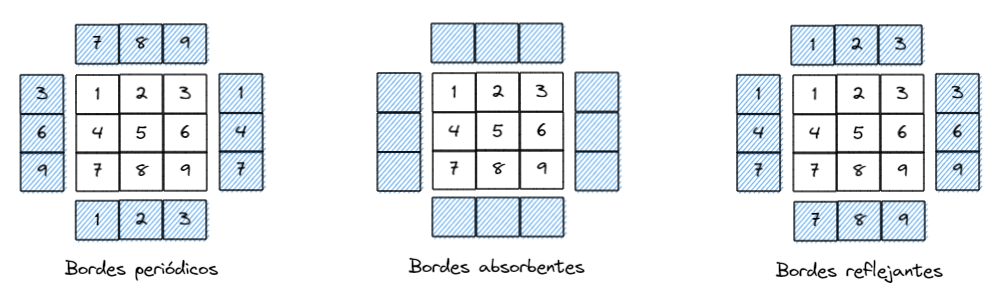
\includegraphics[width=0.8\textwidth]{Imagenes/Tipos_de_borde.PNG}
  \caption{Tipos de borde usuales para autómatas celulares}
  \label{fig:Tipos de borde}
\end{figure}
    
\underline{\textit{Nota:}} Para los objetivos del proyecto implementaremos unicamente bordes del tipo absorbente.

\subsubsection{Conjunto de estados}

Dependiendo del contexto en que estemos implementando nuestro autómata celular, las células podrán adquirir diferentes atributos. Por ejemplo, si consideramos el ejercicio realizado en  \cite{NetLogoFireModel} en el que se modela la propagación del fuego en un bosque se consideran dos estados: los arboles que están quemados de color rojo y los que no se quemaron verde en la figura (\ref{fig:Fuego Netlogo}). Como puede apreciarse en el ejemplo, hay células que cambian de estado en el tiempo.

\begin{figure}[h]
  \centering
    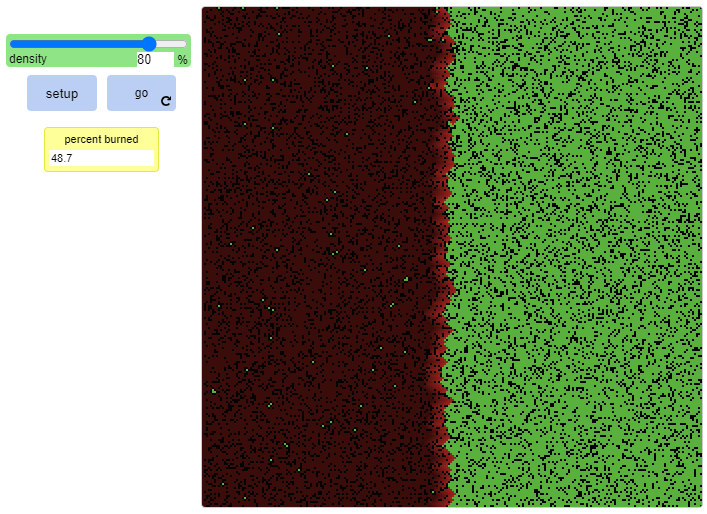
\includegraphics[width=0.4\textwidth]{Imagenes/netlogoEx1.PNG}
  \caption{Modelo del fuego en Netlogo. Captura tomada de \cite{NetLogoFireModel}.}
  \label{fig:Fuego Netlogo}
\end{figure}

\textbf{Definición 1.5.2:} El \textit{conjunto de estados} $\Sigma$ es el conjunto finito de todas las posibles categorias en las que pueden estar las células del espacio $\mathcal{L}$. Cada elemento $\simga$ de $\Sigma$ será conocido como un estado del modelo.

\subsubsection{Vecindades}

Una de las ventajas de trabajar con autómatas celulares es que permiten establecer relaciones entre las células por medio de vecindades. En general no se trabaja con todo el conjunto $\mathcal{V}(x)$ sino que se consideran elementos de cada una de estas familias para conformar un conjunto de vecindades sobre el espacio $\mathcal{L}$. Este conjunto se conoce como un \textit{sistema de vecindades} sobre $\mathcal{L}$.

Generalmente cuando se desarrollan análisis usando autómatas celulares se trabaja con sistemas de vecindades definidos a partir de las vecindades de Moore o de la de Von neumann. 

La vecindad de Von neumann se compone de una célula central y de las que se encuentran a los lados formando así una especie de cruz. De manera formal la vecindad de Von neumann de la celda $i,j$ se define como:

$$\mathcal{V}_V(x_{i,j}) = \{x_{k,l}\mid\abs{i-k}+\abs{j-l}\leq1\text{, con }k,l\in\mathbb{Z}\}$$

Por otro parte tenemos a la vecindad de Moore la cual se define de manera similar a la vecindad de Von neumann. La diferencia entre una y otra radica en que la vecindad de Moore incluye a las células de las diagonales formando un cuadrado. La vecindad de Moore se define  de la célula $i,j$ como:

$$\mathcal{V}_M(x_{i,j}) = \{x_{k,l}\mid\abs{i-k},\abs{j-l}\leq1\text{, con }k,l\in\mathbb{Z}\}$$

En la figura (\ref{fig:Moore - Von neumann}) podemos identificar a las celdas de color verde como las células centrales para cada vecindad y las de color azul como sus vecinos:

\begin{figure}[h]
  \centering
    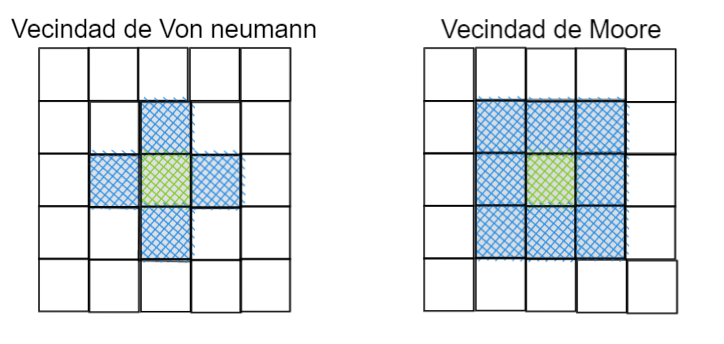
\includegraphics[width=0.5\textwidth]{Imagenes/vecindades.PNG}
  \caption{Vecindades usuales para autómatas celulares}
  \label{fig:Moore - Von neumann}
\end{figure}

\subsubsection{Reglas de evolución}

Las reglas de evolución definen la manera en la que cambian los estados de cada célula teniendo en cuenta el estado de sus vecinos. En general definimos una regla de evolución $\phi$ como sigue:

$$\phi:\Sigma_x\times\overbrace{\Sigma\times\Sigma\times\cdots\times\Sigma}^{N}\longrightarrow\Sigma_x,$$

donde $N$ es la cantidad de vecinos de $x$ y $\Sigma_x$ el conjunto de estados que puede tomar $x$. 

Para determinar la evolución del espacio $\mathcal{L}$ se debe aplicar la regla de evolución simultáneamente sobre cada una de sus células. De ese modo podemos definir una regla global de evolución $\Phi$ como la aplicación de la regla $\phi$ sobre cada una de las células de un espacio $\mathcal{L}$.

Las reglas de evolución pueden ser de dos tipos:

\begin{itemize}
    \item \textbf{Reglas determinísticas}
    
    Son aquellas en las que se define un estado para cada posible combinación de estados en la vecindad. Un ejemplo de esto son las \textbf{reglas de Wolfram} en las que se define la correspondencia entre los estados de una celda $x$ y sus vecinos con el estado posterior de la celda $x$. Consideremos como caso particular a la regla 30 en la que se define la siguiente correspondencia:
    
    \begin{figure}[h]
      \centering
        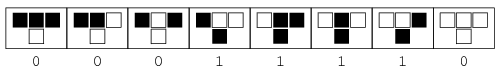
\includegraphics[width=0.7\textwidth]{Imagenes/regla30.PNG}
      \caption{Regla 30. Captura tomada de \cite{rule30}}
      \label{fig:Regla30}
    \end{figure}
    
    Al tratarse de una regla sobre un espacio 1-dimensional los vecinos de cada célula son los que se encuentran a lados izquierdo y derecho, como se ve en la figura (\ref{fig:Regla30}). En este caso el conjunto de estados es de la forma $\Sigma=\{0,1\}$. En la figura (\ref{fig:regla30en15y250}) podemos apreciar la evolución del espacio de células $\mathcal{L}$ en 15 y 250 iteraciones respectivamente para la aplicación de la regla 30 denotada como $\phi_{30}$.
    
    \begin{figure}[htbp]
        \centering
        \subfigure[Evolución del espacio $\mathcal{L}$ luego de 15 iteraciones]{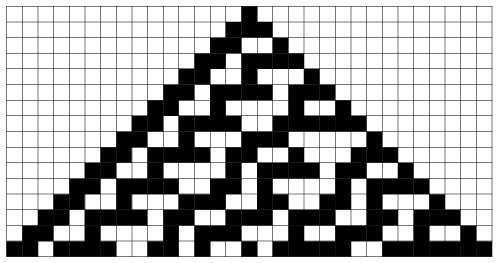
\includegraphics[width=60mm]{Imagenes/regla30en15.PNG}}
        \subfigure[Evolución del espacio $\mathcal{L}$ luego de 250 iteraciones]{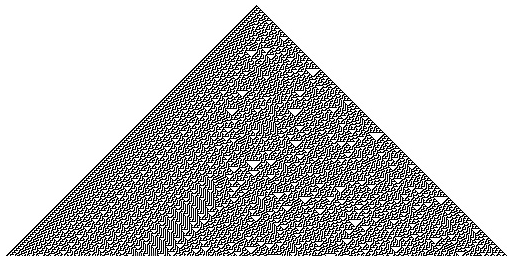
\includegraphics[width=60mm]{Imagenes/regla30en250.PNG}}
        \caption{Evoluciones al aplicar la regla 30 de Wolfram. Captura tomada de \cite{rule30}}\label{fig:regla30en15y250}
    \end{figure}
    
    \item \textbf{Reglas totalísticas}
    
    A diferencia de las reglas determinísticas, las reglas totalísticas no establecen una correspondencia directa entre estados y combinaciones de vecindades, sino que en su lugar utilizan un componente probabilístico. Esto significa que dependiendo de la combinación, la célula sobre la que se aplica la regla puede tomar un estado de un subconjunto del conjunto de estados $\Sigma$. 
    
    Existe un subtipo de este tipo de reglas conocido como las reglas semi-totalísticas, en las que el subconjunto que se considera para la evolución de la célula sobre la que se aplica la regla depende del estado de la misma célula. De ese modo:
    
    \begin{align*}
        \phi:\Sigma_x\times\overbrace{\Sigma\times\Sigma\times\cdots\times\Sigma}^{N}&\longrightarrow \left\{ \begin{array}{cc}
        \sigma_1 \subseteq \Sigma_x & \text{si el estado de }x\text{ es }s_1 \\
        \sigma_2 \subseteq \Sigma_x & \text{si el estado de }x\text{ es }s_2 \\
        \vdots & \vdots \\
        \sigma_k \subseteq \Sigma_x & \text{si el estado de }x\text{ es }s_k
        \end{array} \right. ,
    \end{align*}
    
    donde $k$ es la cantidad de posibles estados que puede tomar $x$.
\end{itemize}

A pesar de que las reglas determinísticas pueden generar resultados interesantes su implementación computacional no resulta muy cómoda, sobre todo si consideramos espacios de células de más de una dimensión. De acuerdo con \cite{alfons2010}, la cantidad de posibles combinaciones o reglas que se pueden definir si usáramos las del tipo determinista serían:

$$N_r=\#\Sigma^{\#\Sigma^N},$$

donde $\#\Sigma$ es la cantidad de estados en $\Sigma$ y $N$ es la cantidad de vecinos que se consideran en el sistema de vecindades. Por ejemplo, para el caso de la regla 30 la cantidad de reglas que se pueden definir es igual a $2^{2^2}=16$. Esto representa una complicación al trabajar con espacios de más de una dimensión por lo que para los propósitos del proyecto nos enfocaremos únicamente sobre las reglas totalísticas y para ser más específicos sobre las reglas semi-totalísticas, esto debido al contexto de nuestro proyecto.

Una vez aclarados todos los conceptos que abarcan los autómatas celulares podemos dar una definición formal de ellos:

\textbf{Definición 1.5.3:} Un autómata celular es una la tupla de la forma  $A=(\mathcal{L},\Sigma,\mathcal{N}(\mathcal{L}),\phi)$ con $\mathcal{N}(\mathcal{L})$ un sistema de vecindades sobre $\mathcal{L}$.
